\documentclass[12pt]{beamer}
\usepackage{breqn}
\usepackage[brazilian,hyperpageref]{backref}
\usepackage[num]{abntex2cite}		% Citações padrão ABNT
\usepackage[utf8]{inputenc}
\usepackage[portuguese]{babel}
\usepackage{colortbl}
\usepackage{color}
\usepackage{amsmath}
\usepackage{url}
\usepackage{hyperref}
\usepackage{beamerthemeshadow}
\usepackage{verbatim}
\usepackage{listings}
\usepackage{tikz}

\graphicspath{{./images/}}
\citebrackets[]

\setbeamertemplate{bibliography item}{\insertbiblabel}
\setbeamertemplate{caption}[numbered]

\renewcommand{\backrefpagesname}{Citado na(s) página(s):~}
% Texto padrão antes do número das páginas
\renewcommand{\backref}{}
% Define os textos da citação
\renewcommand*{\backrefalt}[4]{}
    %\ifcase #1 %
        %Nenhuma citação no texto.%
    %\or
        %Citado na página #2.%
    %\else
        %Citado #1 vezes nas páginas #2.%
    %\fi}%

\beamertemplatenavigationsymbolsempty% tira os elementos de navegação da parte de baixo
%\setbeamertemplate{footline}{}%remove o autor e o título da parte de baixo

\addtobeamertemplate{navigation symbols}{}{%
    \usebeamerfont{footline}%
    \usebeamercolor[black]{footline}%
    \hspace{1em}%
    \insertframenumber/\inserttotalframenumber%
}

\usetheme{Frankfurt}
\usecolortheme{orchid}

\author{Victor Emanuel Almeida}
\title{Arduino}
\subtitle{Dia 1, conceitos básicos e criando o primeiro projeto}
\date{11 de maio de 2023}
\institute{UNIOESTE}
\logo{
\includegraphics[height=1cm]{logo_unioeste.jpg}}

\definecolor{dkgreen}{rgb}{0,0.6,0}
\definecolor{gray}{rgb}{0.5,0.5,0.5}
\definecolor{mauve}{rgb}{0.58,0,0.82}
\definecolor{laranja_claro}{rgb}{1,0.9,0.5}
\definecolor{laranja_escuro}{rgb}{1,0.5,0.2}
\definecolor{azul_claro}{rgb}{0.5,0.9,1}

\lstset{frame=tb,
    language=C++,
    frame=tb,
    aboveskip=3mm,
    belowskip=3mm,
    showstringspaces=false,
    columns=flexible,
    basicstyle={\small\ttfamily},
    numbers=left,
    numberstyle=\tiny\color{gray},
    keywordstyle=\color{blue},
    commentstyle=\color{dkgreen},
    stringstyle=\color{mauve},
    breaklines=true,
    breakatwhitespace=true,
    xleftmargin=.05\textwidth,
    xrightmargin=.05\textwidth,
    tabsize=4,
}

\begin{document}
\frame{\titlepage}

\begin{frame}
    \frametitle{Conteúdo}
    \tableofcontents
\end{frame}

\section{Introdução}

\begin{frame}
    \frametitle{Questões}
    \begin{itemize}
        \item Quem nunca fez um projeto com Arduino?
        \item Quem já sabe usar bem o Arduino?
    \end{itemize}
\end{frame}

\begin{frame}
    \frametitle{Conteúdo Open software}
    slides e sketch's disponibilizados em: \url{https://github.com/darkvictor13/AulaArduino}
\end{frame}

\begin{frame}
    \frametitle{O que é Arduino?}

    \begin{itemize}
        \item Empresa italiana que produz placas de prototipagem eletrônica;
        \item Possui um ecossistema de hardware e software;
        \begin{itemize}
            \item\textbf{Hardware}: +100 produtos (placas, acessórios, shields, etc)\cite{site_arduino};
            \item\textbf{Software}:
            \begin{itemize}
                \item Linguagem de programação adaptada do C++;
                \item IDE versões 1 e 2;
                \item Cloud;
            \end{itemize}
        \end{itemize}
        \item Hardware e software livre;
        \item Foco em prototipagem rápida e educacional;
        \item Comunidade ativa e grande;
    \end{itemize}
\end{frame}

\section{Hardware}
\begin{frame}[allowframebreaks]
    \frametitle{Tipos de arduino}

    Como comentado anteriormente, a empresa Arduino possui uma grande variedade de placas,
    cada uma para uma funcionalidade diferente.
    
    A seguir, serão apresentadas algumas delas

    \framebreak%

    \begin{figure}
        \centering
        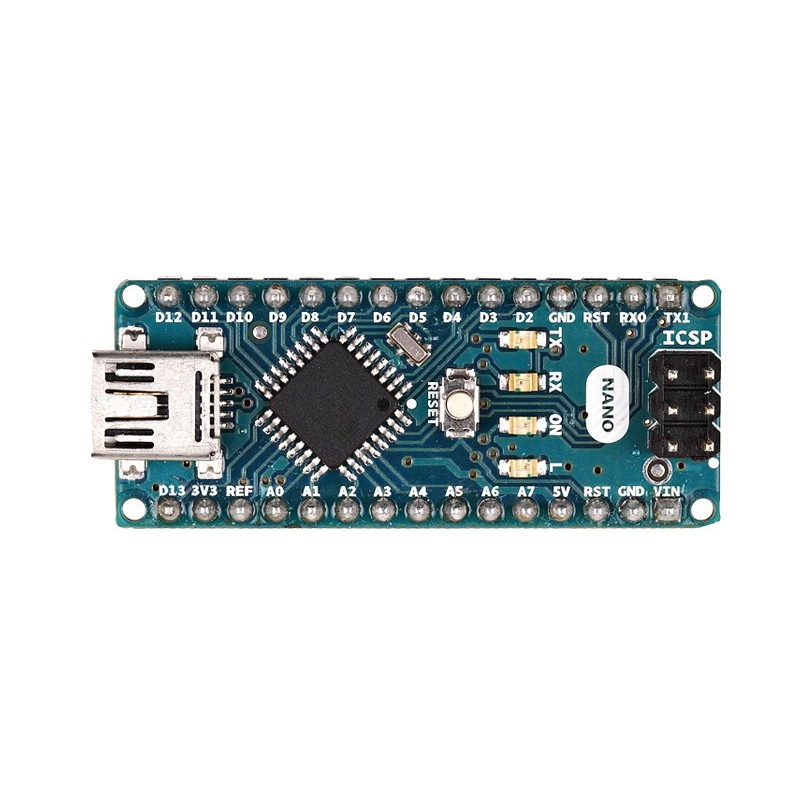
\includegraphics[height=.68\textheight]{arduino_nano}
        \caption{Arduino Nano}
    \end{figure}

    \framebreak%
    \begin{figure}
        \centering
        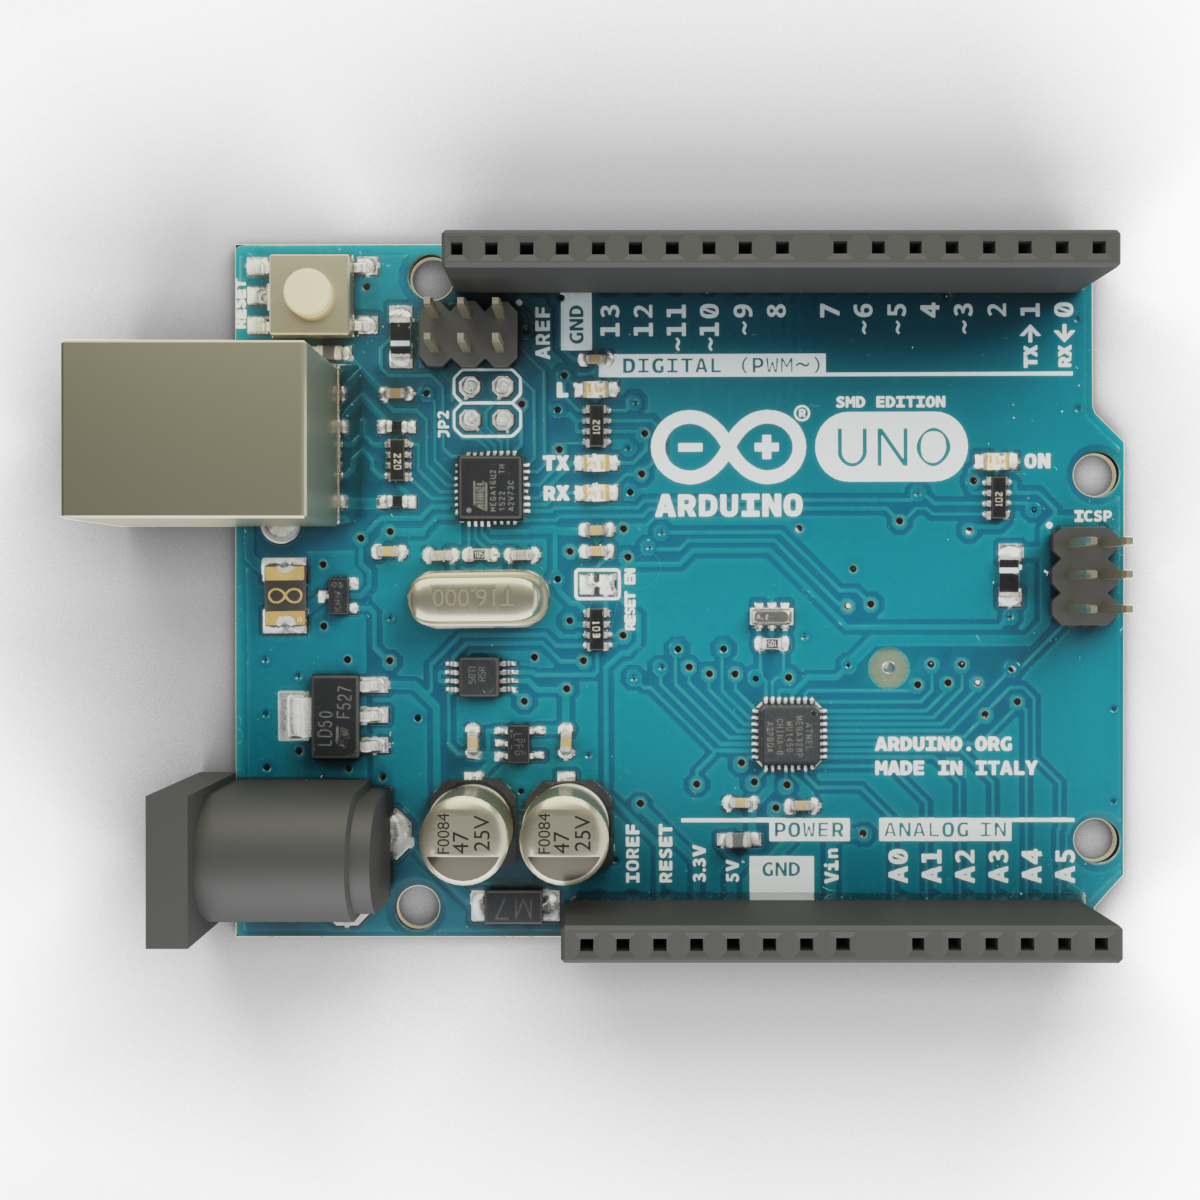
\includegraphics[height=.68\textheight]{arduino_uno}
        \caption{Arduino Uno}
    \end{figure}

    \framebreak%
    \begin{figure}
        \centering
        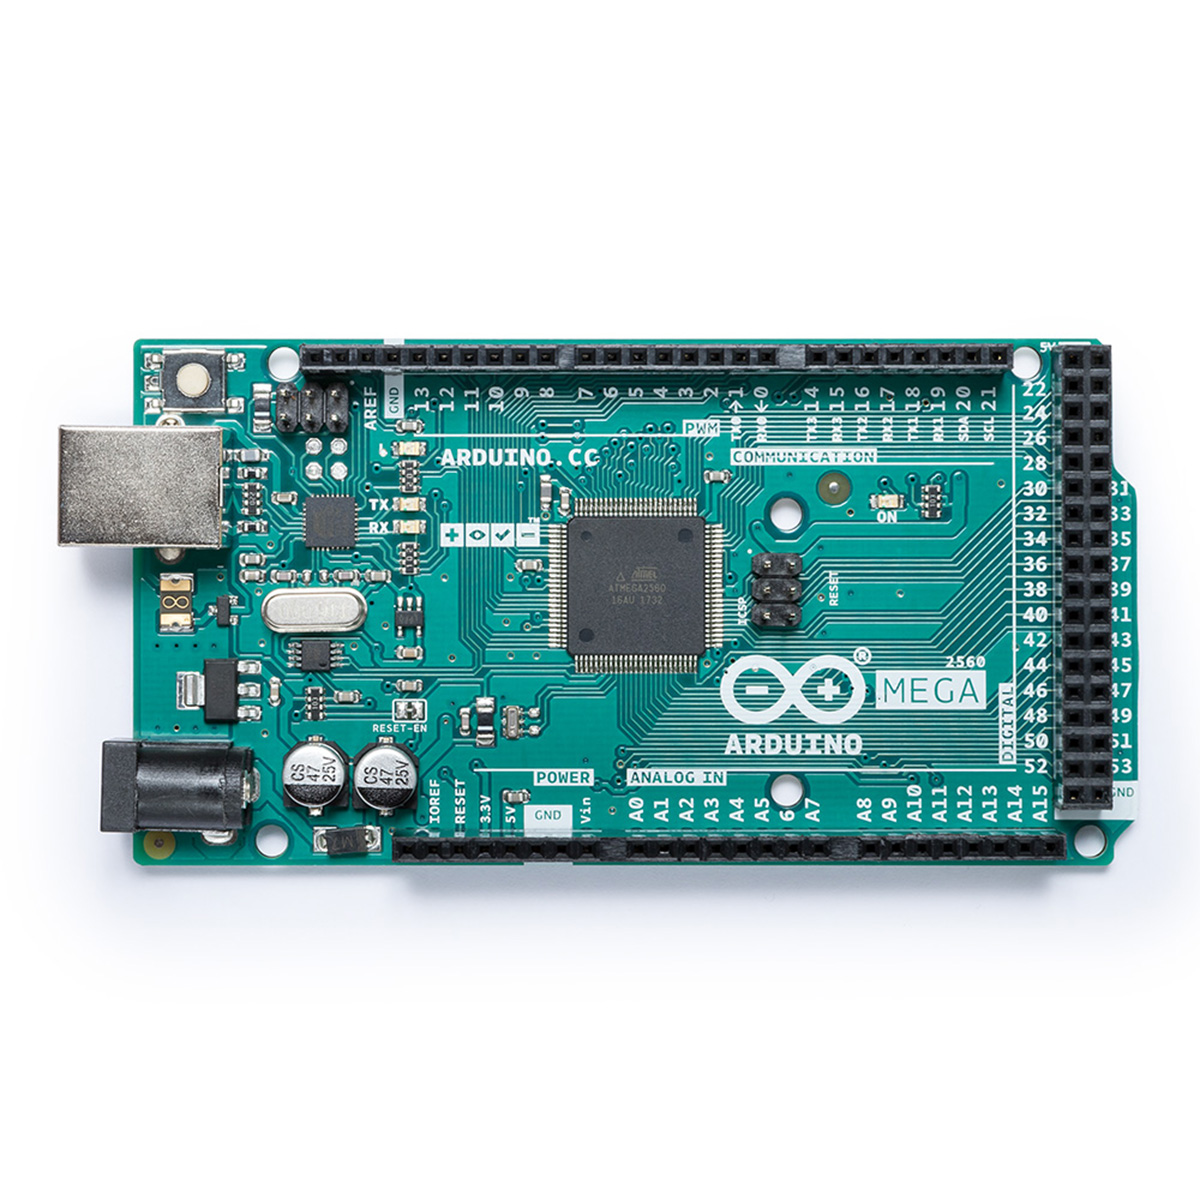
\includegraphics[height=.68\textheight]{arduino_mega}
        \caption{Arduino Mega}
    \end{figure}
\end{frame}

\begin{frame}
    \frametitle{Partes do Arduino Mega}

    \begin{figure}
        \centering
        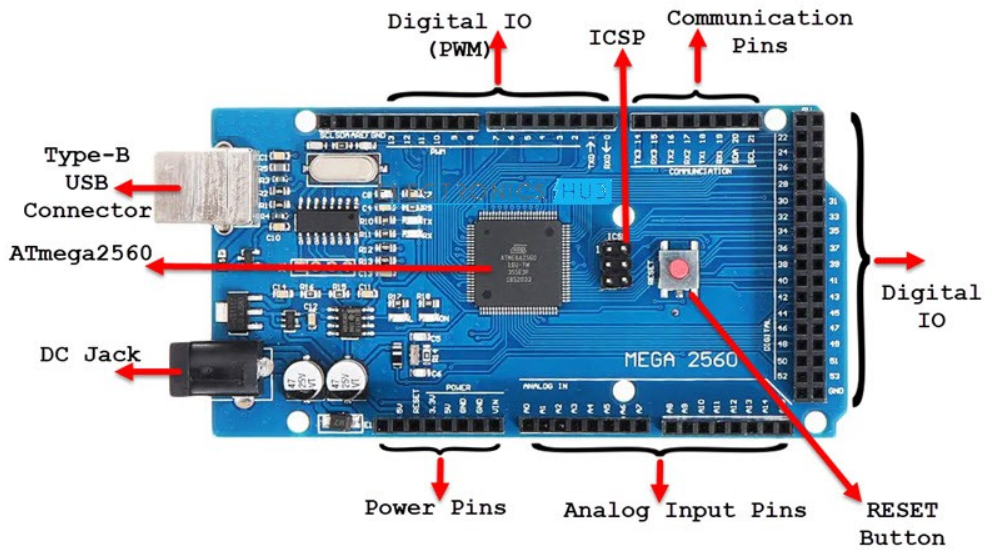
\includegraphics[height=.68\textheight]{partes_arduino_mega}
        \caption{Arduino Mega}
    \end{figure}

\end{frame}

\begin{frame}
    \frametitle{Pinout}
    \begin{figure}
        \centering
        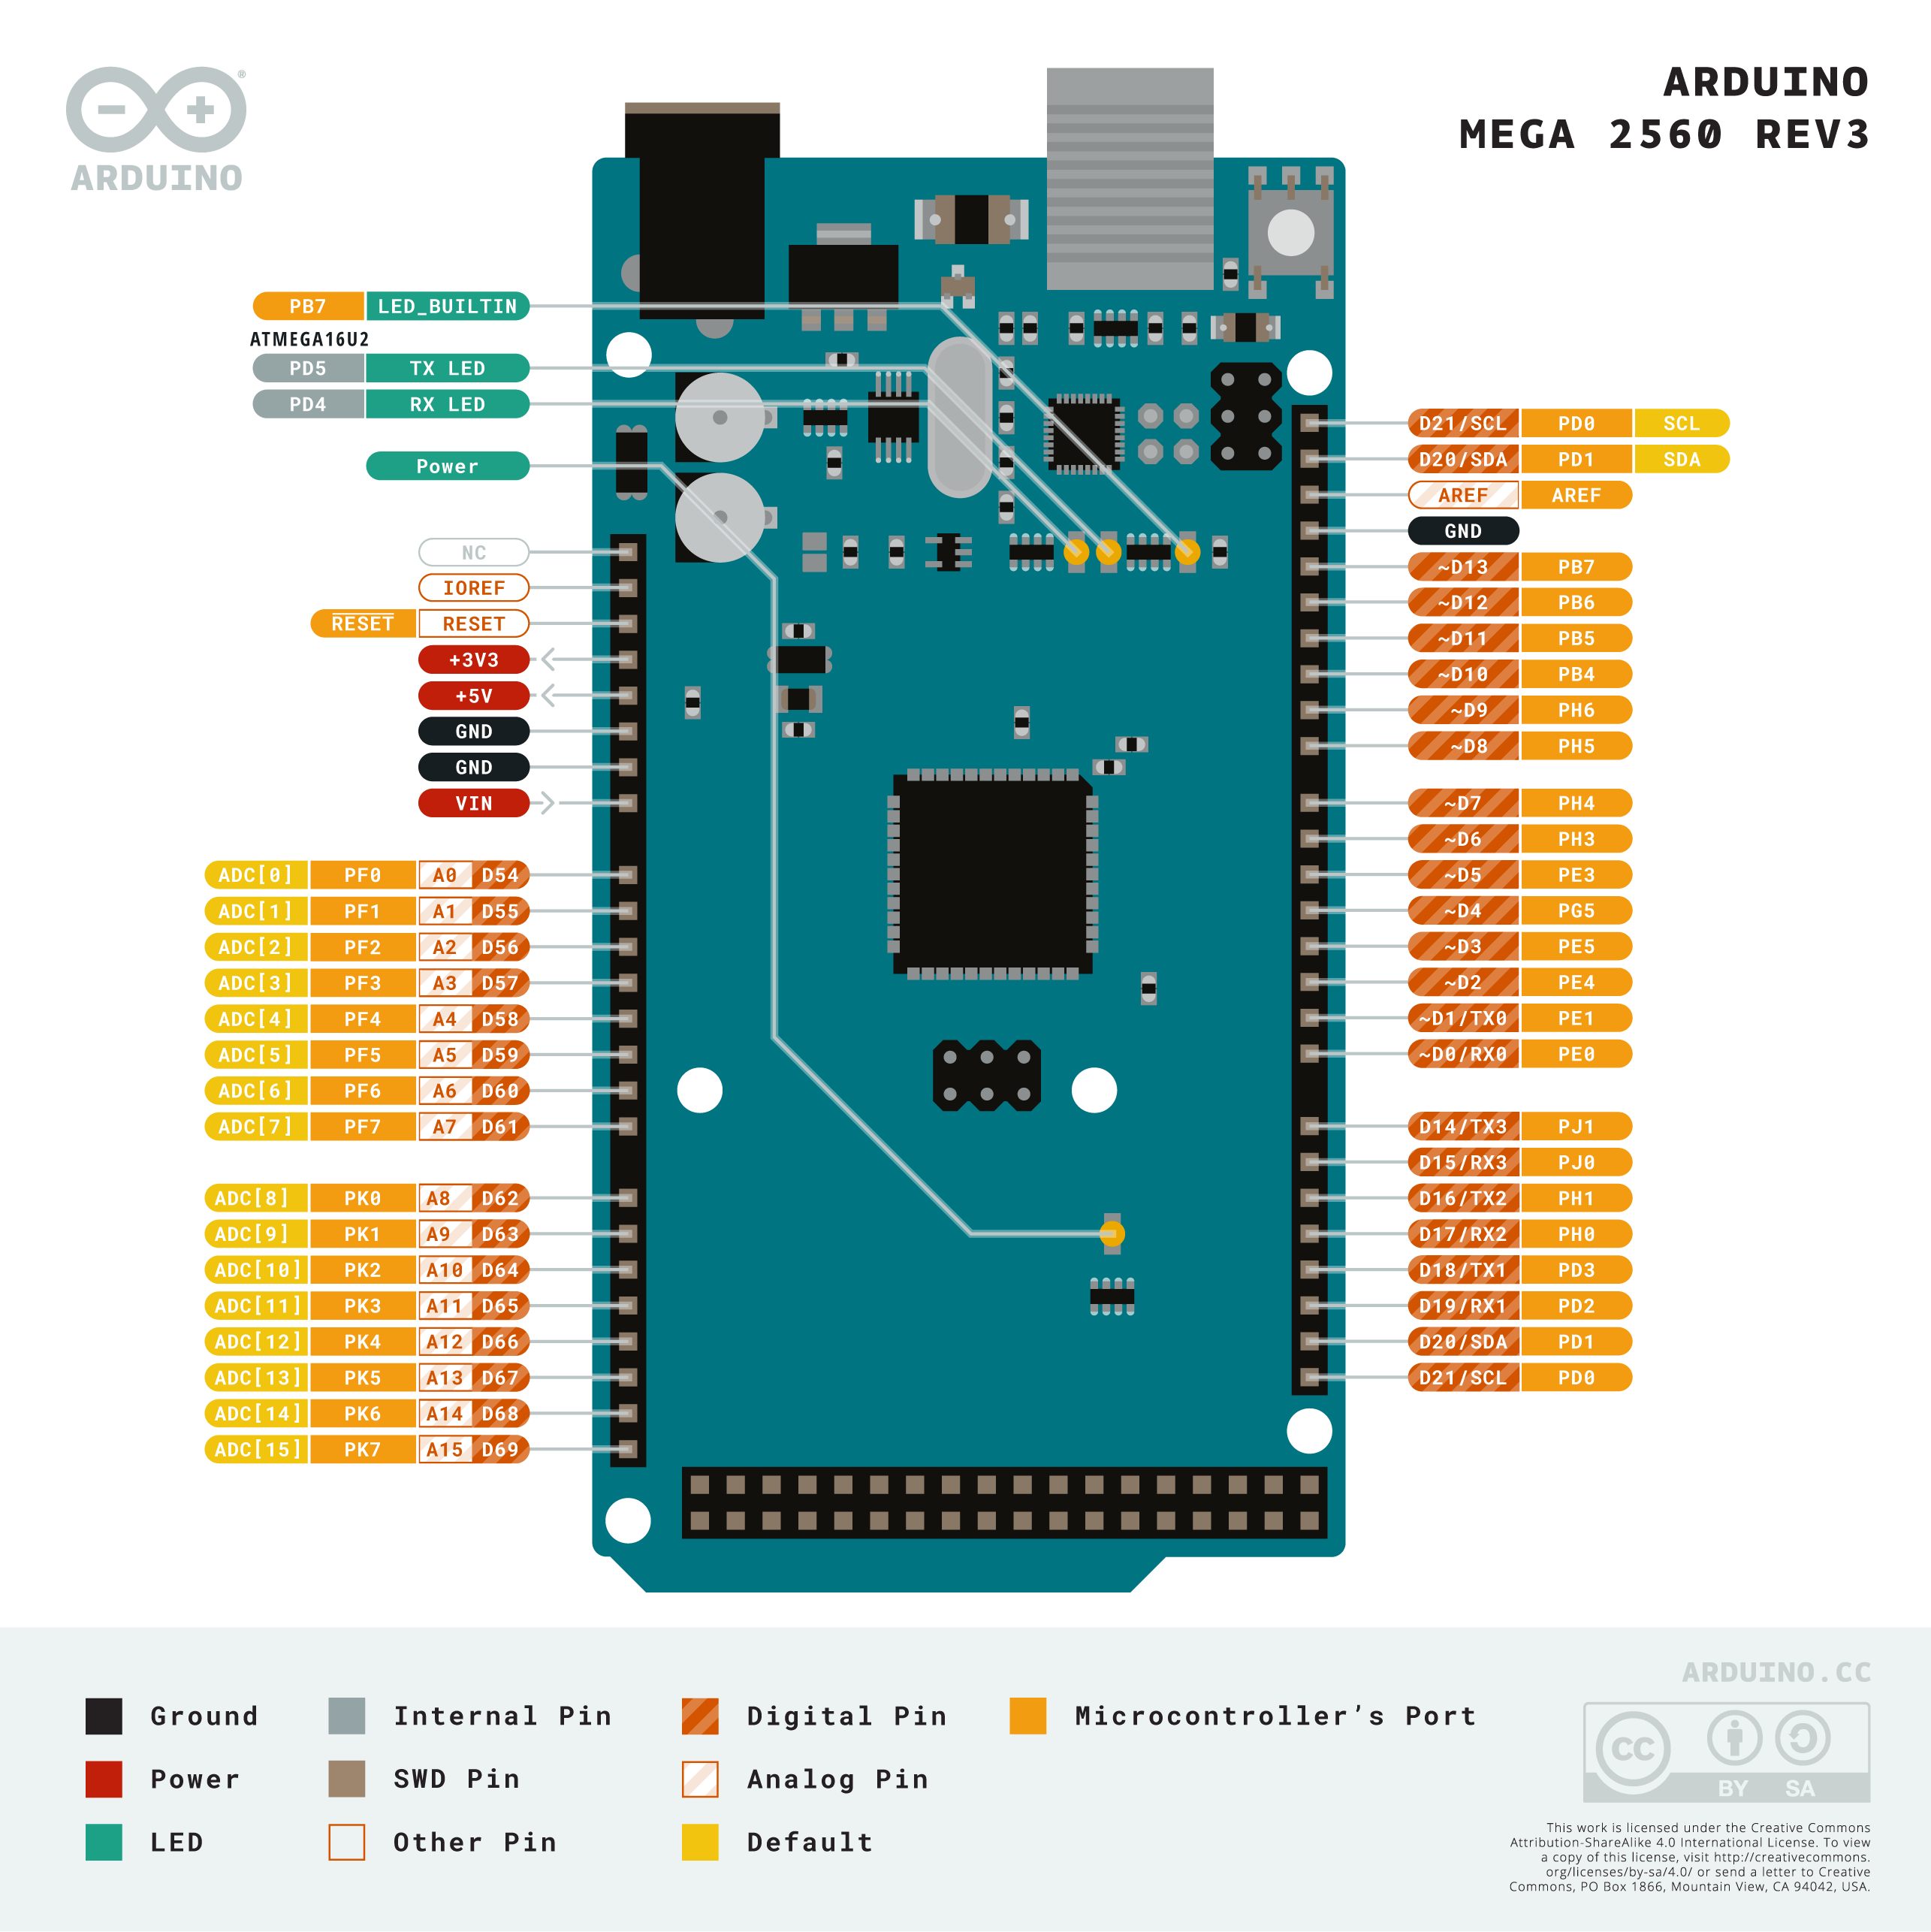
\includegraphics[height=.68\textheight]{Pinout-Mega2560}
        \caption{Pinout do Arduino Mega}
    \end{figure}
\end{frame}

% TODO Fazer um slide mostrando cada parte de uma placa arduino
% Microcontrolador, portas, etc

\section{Software}

\begin{frame}
    \frametitle{Ambientes de desenvolvimento}
    \begin{itemize}
        \item Arduino IDE\@;
        \item PlatformIO\@;
        \item Fazer na mão;
        \item Outros;
    \end{itemize}
\end{frame}

\begin{frame}
    \frametitle{Arduino IDE}

    \begin{itemize}
        \item Temos a versão 1 e 2;
        \item Melhorias da versão 2 (muito baseada no VSCode):
        \begin{itemize}
            \item Autocompletar;
            \item Gerenciamento de bibliotecas;
            \item Possibilidade de abrir arquivos de bibliotecas (Ctrl + Click);
            \item Integração com Git;
        \end{itemize}
    \end{itemize}
\end{frame}

\begin{frame}[allowframebreaks]
    \frametitle{Instalação}

    \begin{itemize}
        \item Windows:
            \begin{itemize}
                \item Vá para o site do Arduino \url{https://www.arduino.cc/en/software\#future-version-of-the-arduino-ide}
                \item Escolher a opção \textbf{Windows 10 and newer};
            \end{itemize}

        \framebreak%
        \begin{figure}
            \centering
            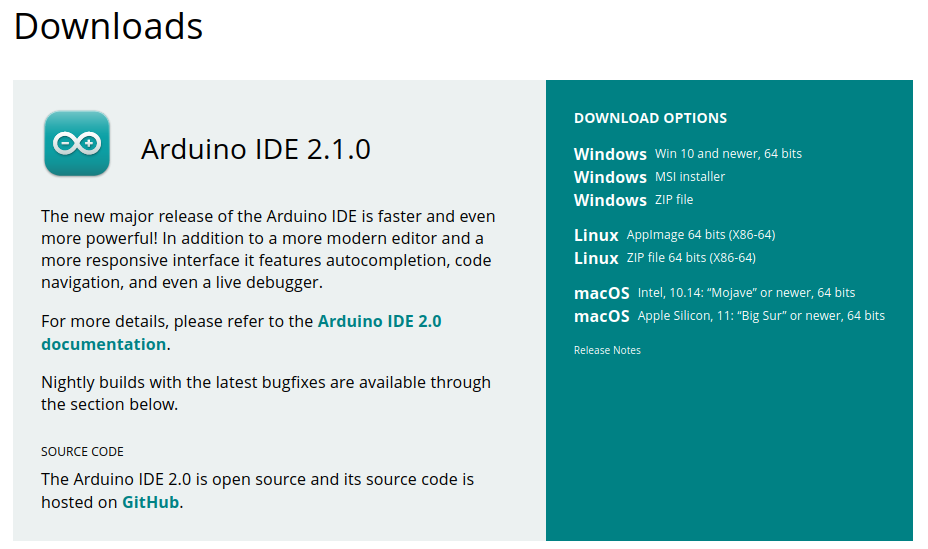
\includegraphics[height=.68\textheight]{download_arduino_ide}
            \caption{Tela de Download}
        \end{figure}

        \framebreak%
        \begin{figure}
            \centering
            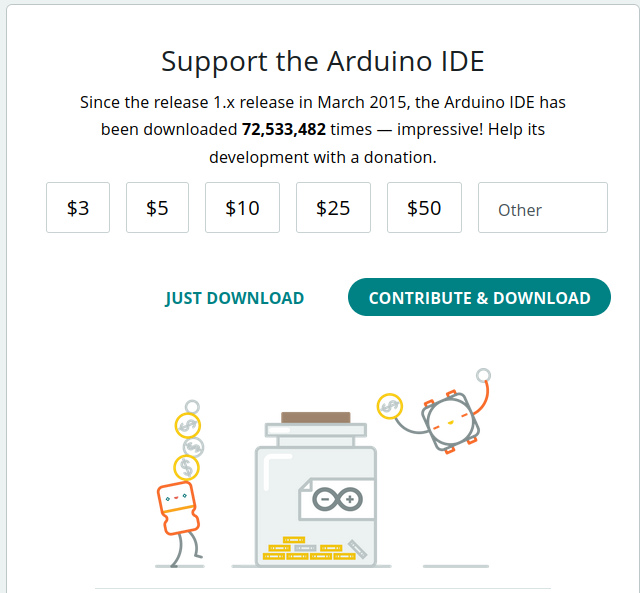
\includegraphics[height=.68\textheight]{download}
            \caption{Tela de confirmação de download}
        \end{figure}


        \framebreak%
        \item Linux:
        \begin{itemize}
            \item Arch: \texttt{paru -S arduino-ide-bin};
            \item Outras distros (Ubuntu, Mint, etc):
            \begin{itemize}
                \item Vá para o site do Arduino \url{https://www.arduino.cc/en/software\#future-version-of-the-arduino-ide}
                \item Escolha a opção \textbf{AppImage 64 bits};
                \item Dê permissão de execução para o arquivo baixado \texttt{chmod +x arduino-ide_2.1.0_Linux_64bit.AppImage};
                \item Mova o arquivo para a pasta de binários \texttt{mv arduino-ide_2.1.0_Linux_64bit.AppImage /usr/bin/arduino-ide};
            \end{itemize}
        \end{itemize}
    \end{itemize}
\end{frame}

\begin{frame}
    \frametitle{Utilizando a IDE}

    \begin{figure}
        \centering
        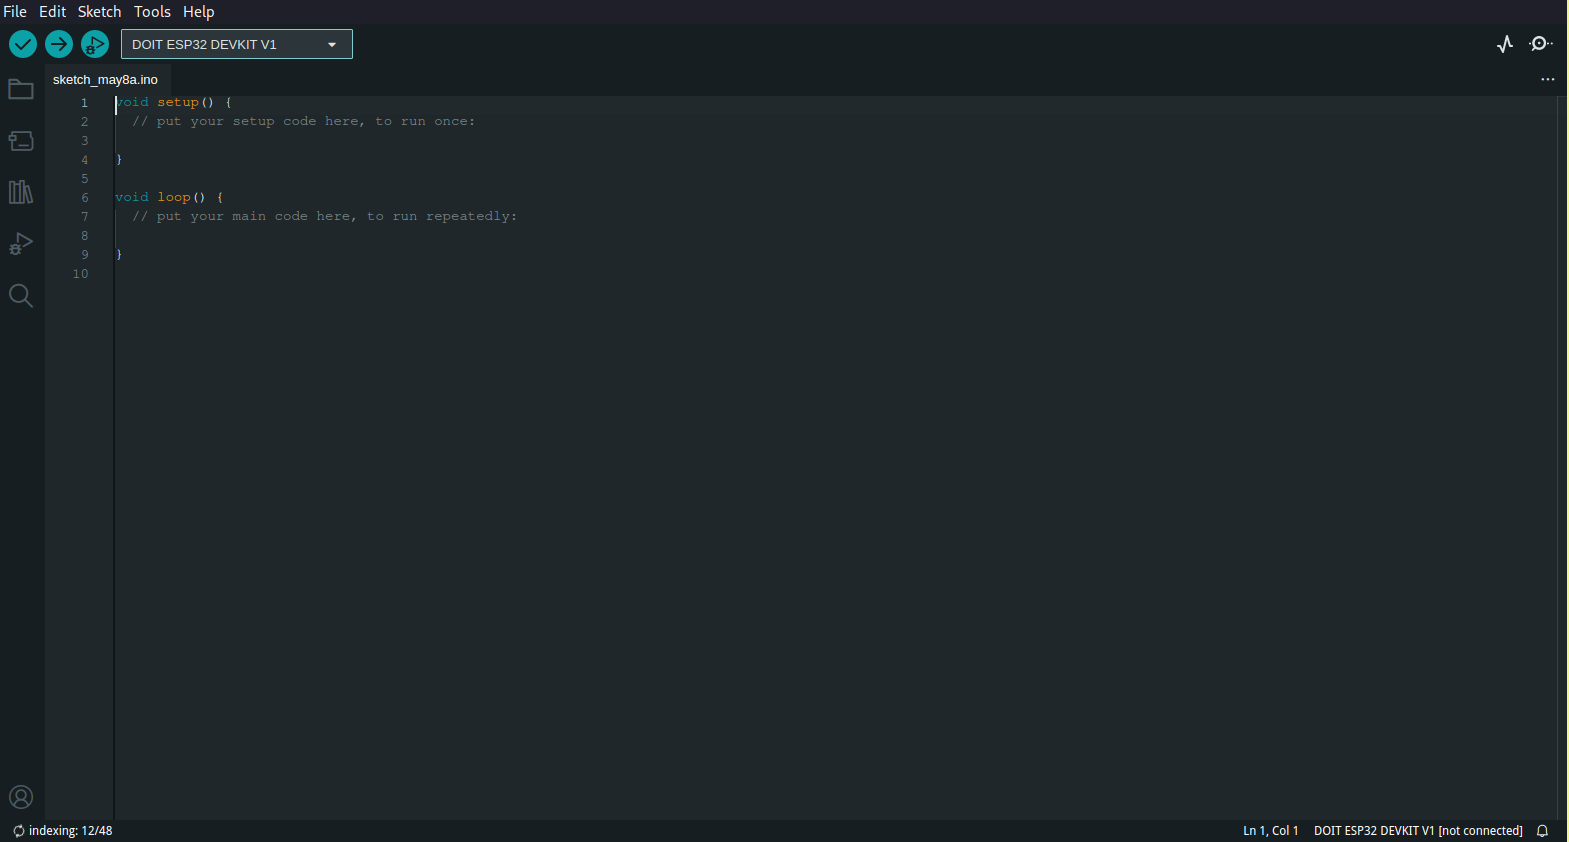
\includegraphics[height=.68\textheight]{ide}
        \caption{Tela inicial da IDE}
    \end{figure}

\end{frame}

\begin{frame}[t,fragile]
    \frametitle{Estrutura do programa}
    \begin{lstlisting}
#include <Arduino.h>

void setup() {
    // func executada uma vez
    // quando o arduino liga
}

void loop() {
    // func executada continuamente
    // enquanto o arduino estiver ligado
    // executada depois do setup
}
    \end{lstlisting}
\end{frame}

\begin{frame}
    \frametitle{Exemplos de programas para serem implementados}

    \begin{itemize}
        \item Hello World;
        \item Blink LED interno;
        \item Blink LED externo;
    \end{itemize}

\end{frame}

\section{Considerações Finais}
\begin{frame}[allowframebreaks]
    \frametitle{Referências}
    \bibliography{ref}
\end{frame}

\begin{frame}
    \frametitle{Contato}
    \centering
    \url{archvictor@protonmail.com}
    \url{https://github.com/darkvictor13}
\end{frame}

\end{document}
